\subsection{Kommunikationsmöglichkeiten}
\label{subsec:manual}
In diesem Kapitel wird erläutert, wie die beiden Kommunikationsmittel der Wetterstation zu benutzen sind und worauf zu achten ist.\\

\subsubsection{USB-to-Computer}
\label{subsubsec:usbtocomputer}
Diese serielle Verbindung wurde hauptsächlich für Debbuging- und Verifikations-Zwecke verwendet. Sie bietet aber auch eine Möglichkeit, als User mit der Wetterstation direkt zu kommunizieren.

\paragraph{Setup}
\label{para:puttysetup}
Um die Verbindung erstellen zu können muss zuerst PuTTY (Tab. \ref{tab:toolchain}) und noch der FTDI-Driver (zu finden auf \url{https://www.ftdichip.com/Drivers/VCP.htm}) auf dem Computer installiert werden. Sind diese beiden Dinge abgeschlossen und das Target angeschlossen, muss noch der COM-Port des FTDI-Chips unter Geräte-Manager/Anschlüsse(COM\&LPT) ausgelesen werden. Wie in der Abb. \ref{fig:einstellungenputty} zu sehen, sollte als Connection Type Serial gewählt, der COM-Port und die Baudrate eingetragen werden. Als Baudrate 9600 Baud verwenden, ansonsten funktioniert es nicht. Zusätzlich sollten noch Einstellungen bei den Parity und Stop Bits berücksichtigt werden (siehe Abb. \ref{fig:parityundstopbits}). Es gibt kein Parity Bit, ein Stop Bit und acht Daten Bits. Danach kann der Port geöffnet werden.\\

\begin{minipage}[b][6.5cm][t]{0.3\textwidth}
\centering
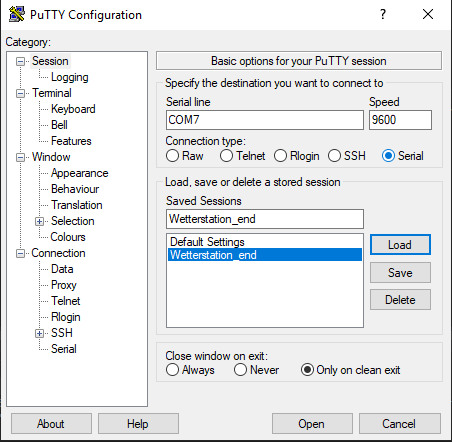
\includegraphics[width=0.5\textwidth]{../../graphics/putty/einstellungen.PNG}
\label{fig:einstellungenputty}
\captionof{figure}{Einstellungen}}
\end{minipage}
\begin{minipage}[b][6.5cm][t]{0.3\textwidth}
\centering
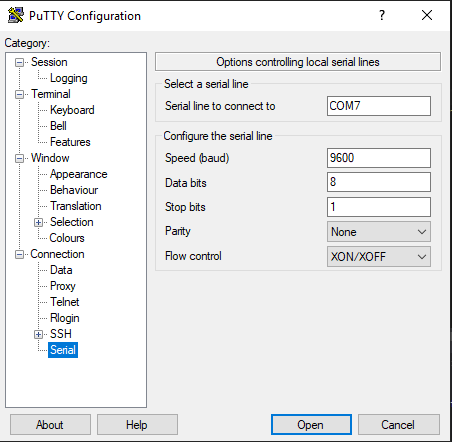
\includegraphics[width=0.5\textwidth]{../../graphics/putty/einstellungen_bits.PNG}
\label{fig:parityundstopbits}
\captionof{figure}{Parity und Stop Bits}
\end{minipage}

Wurde das Target geresetet und der Port mittels PuTTY geöffnet, dann \textbf{muss} eine beliebige Taste gedrückt werden, damit die Wetterstation anfängt zu initialisieren. Hat der DS3231 einmal seine Speisung verloren, werden die Zeitdaten zu Beginn manuell zurückgesetzt. Anschließend kommt für die Entsperrung der SIM-Karte noch die Pin-Eingabe.\\

Sobald alles initialisiert wurde und die Wetterstation sich im Loop befindet (Kapitel \ref{subsec:uml}), können einige Abfragen über den Computer getätigt werden:\\
\begin{itemize}
	\item show battery
	\item show temp
	\item show humi
	\item show press
	\item show rainfall
	\item show wind
	\item show gps
	\item show light
	\item read sms
	\item delete sms
	\item delete all sms
\end{itemize}
Falls ein unbekannter Command geschickt wird, wird \textit{unknown command} von der Wetterstation zurückgesendet. Diese Commands sind leicht erweiterbar, da die Klasse CommandLineInterface alle Objektreferenzen von der Main bekommen hat. Sie hat also Zugriff auf alle in der Main instanzierten Instanzen.\\

\subparagraph{Beachte:}
Nach der Initialisierung sollte vor jeder Eingabe eine beliebige Taste gedrückt werden, um der Wetterstation mitzuteilen, dass der User etwas abfragen möchte.\\

\subsubsection{SMS-Abfrage}
\label{subsubsec:smsAbrage}
Für die SMS-Abfrage von einem Mobiltelefon oder Smartphone werden automatische Rückantworten von der Wetterstation nach Erhalt einer SMS generiert. Bei einem unbekannten Command wird \textit{unknown command} zurückgesendet. Bei \textbf{Data}\footnote{data und DATA funktionieren auch} wird eine Nachricht in der folgenden Struktur zurückgesendet.
\begin{itemize}
	\item[ ] Datum Uhrzeit
	\item[ ] Temperatur [C]
	\item[ ] Luftfeuchtigkeit [\%]
	\item[ ] Druck [hPa]
	\item[ ] Beleuchtungsstärke [lux]
	\item[ ] Regenmenge [l/m2]
	\item[ ] Windgeschwindigkeit [m/s]
	\item[ ] Windstärke [Bft]
	\item[ ] Windrichtung
\end{itemize}
Die GPS-Koordinaten sind aktuell nur über das USB-Interface abfragbar. \\
